\documentclass{article}
\usepackage{amsmath}
\usepackage{graphicx}
\usepackage[most]{tcolorbox}
\usepackage{listings}
\usepackage{xcolor}

\lstdefinelanguage{CSS}{
    keywords={color, background-color, margin, padding, border},
    sensitive=false,
    morecomment=[l]{//},
    morestring=[b]",
}

\lstdefinelanguage{TypeScript}{
    keywords={import, from, class, extends, public, private, string, number, console, log, export, const, let, return, new},
    sensitive=true,
    morecomment=[l]{//},
    morecomment=[s]{/*}{*/},
    morestring=[b]",
    morestring=[b]',
    morestring=[b]`
}

\lstset{
    basicstyle=\ttfamily\footnotesize,
    keywordstyle=\color{blue}\bfseries,
    stringstyle=\color{red},
    commentstyle=\color{green!70!black},
    numbers=left,
    numberstyle=\tiny\color{gray},
    stepnumber=1,
    numbersep=10pt,
    backgroundcolor=\color{gray!10},
    frame=single,
    breaklines=true,
    showstringspaces=false,
    tabsize=2,
    captionpos=b
}

\title{Concepts Fondamentaux d'Angular}
\author{}
\date{}

\begin{document}

\maketitle

\section*{Définition d'Angular}

Angular est un framework open-source développé par Google pour la création d'applications web dynamiques. Il repose sur TypeScript et permet de structurer les applications de manière modulaire grâce à une architecture basée sur les composants, les services et les modules. Angular facilite la gestion des données, l'interaction avec des APIs, la gestion des états et la navigation au sein des applications web complexes.


\begin{tcolorbox}[colframe=black!70, colback=white, title=Figure 1: Logo d'Angular, fonttitle=\bfseries]
\centering

\includegraphics[width=0.5\textwidth]{images/Angular_full_color_logo.svg.png}
\end{tcolorbox}


\section*{Architecture d'Angular}

L’architecture d’Angular repose sur une séparation claire des responsabilités pour garantir la scalabilité et la maintenance des applications. Les principaux blocs de cette architecture sont : les \textbf{modules}, les \textbf{composants}, les \textbf{services}, et d'autres entités comme les \textbf{directives} et les \textbf{pipes}.
\begin{tcolorbox}[colframe=black!70, colback=white, title=Figure 2: Architecture d'Angular, fonttitle=\bfseries]
\centering
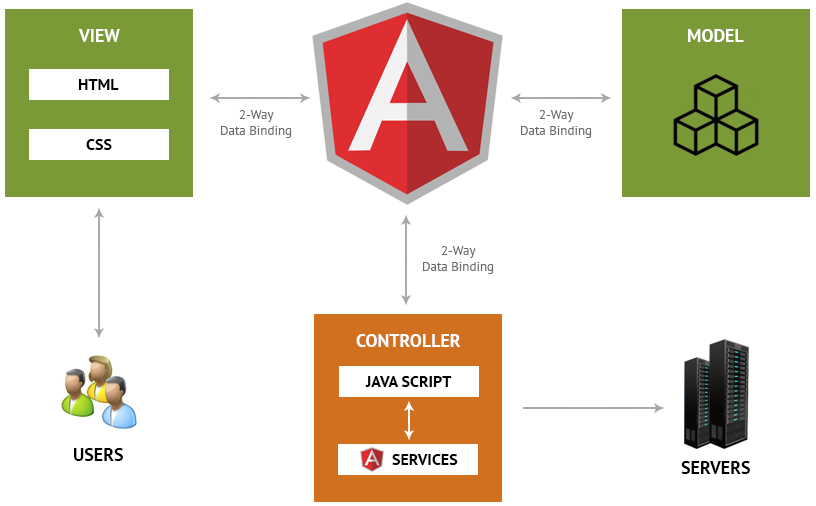
\includegraphics[width=\textwidth]{images/MVC-Architecture-is-Perfect.jpg}
\end{tcolorbox}
L’objectif de cette section est de comprendre comment ces éléments interagissent entre eux pour former une application Angular cohérente.

\section{Vue d’Ensemble de l’Architecture d'Angular}

Angular suit le \textbf{Modèle Vue Contrôleur (MVC)} amélioré, où :
\begin{itemize}
    \item Les \textbf{composants} gèrent l’affichage et capturent les actions de l’utilisateur.
    \item Les \textbf{services} manipulent les données et la logique métier.
    \item Les \textbf{modules} structurent et organisent les différentes fonctionnalités.
\end{itemize}
\begin{tcolorbox}[colframe=black!70, colback=white, title=Figure 3: Architecture d'Angular, fonttitle=\bfseries]
\centering
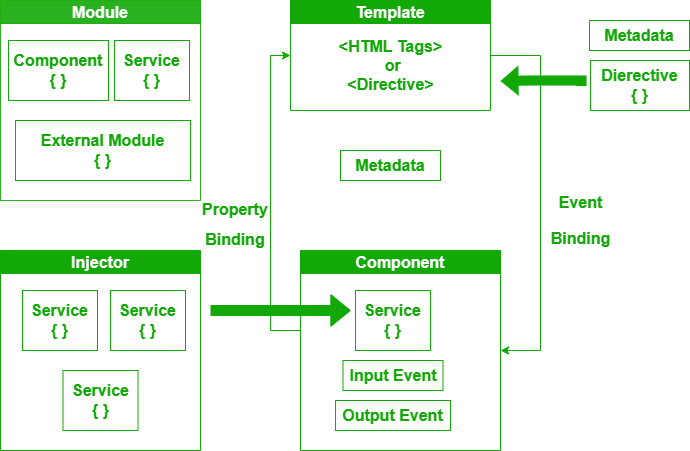
\includegraphics[width=\textwidth]{images/archi.png}
\end{tcolorbox}
Ce modèle favorise une séparation des responsabilités pour un développement modulaire.

\section{Séparation des Responsabilités et Flux d’Information}

\subsection{Les Modules : La Structure Globale}
\begin{itemize}
    \item Les modules définissent le squelette de l’application.
    \item Ils regroupent les composants, services et autres entités.
\end{itemize}

\textbf{Lien avec les autres parties :}  
Les modules servent de conteneurs logiques pour regrouper les fonctionnalités connexes. Par exemple, un module dédié à l’authentification contiendra tous les composants et services liés à la gestion des utilisateurs.

\textbf{Conseil :} Commencez toujours par définir les modules avant de créer les composants et services associés.

\subsection{Les Composants : L’Interface Utilisateur}
\begin{itemize}
    \item Chaque composant représente une partie de l’interface utilisateur (un bouton, un formulaire, une page).
    \item Un composant communique avec les services pour obtenir les données à afficher ou à traiter.
\end{itemize}

\textbf{Flux :}  
Les données transitent \textbf{du service vers le composant}, et les actions utilisateur remontent \textbf{du composant vers le service}.

\textbf{Conseil :} Une fois que le module est configuré, commencez à créer les composants pour concevoir l’interface utilisateur.

\subsection{Les Services : La Logique Métier et les Données}
\begin{itemize}
    \item Les services sont des classes dédiées à la gestion des données et des processus métiers.
    \item Ils utilisent souvent le module HTTP pour communiquer avec des API externes.
\end{itemize}

\textbf{Flux :}  
Les services récupèrent ou manipulent les données, puis les transmettent aux composants.

\textbf{Conseil :} Après avoir défini le modèle de données (interfaces/classes), développez les services pour centraliser la logique métier.

\section{Exemple de Flux d’Information en Trois Étapes}

\begin{enumerate}
    \item \textbf{Définition des Modules :}  
    Créez un module pour une fonctionnalité spécifique (e.g., gestion des produits).
    \item \textbf{Création des Services :}  
    Implémentez un service qui récupère les données des produits via une API.
    \item \textbf{Conception des Composants :}  
    Développez un composant qui utilise le service pour afficher une liste de produits.
\end{enumerate}
\begin{tcolorbox}[colframe=black!70, colback=white, title=Figure 4:  Flux d’Information, fonttitle=\bfseries]
\centering
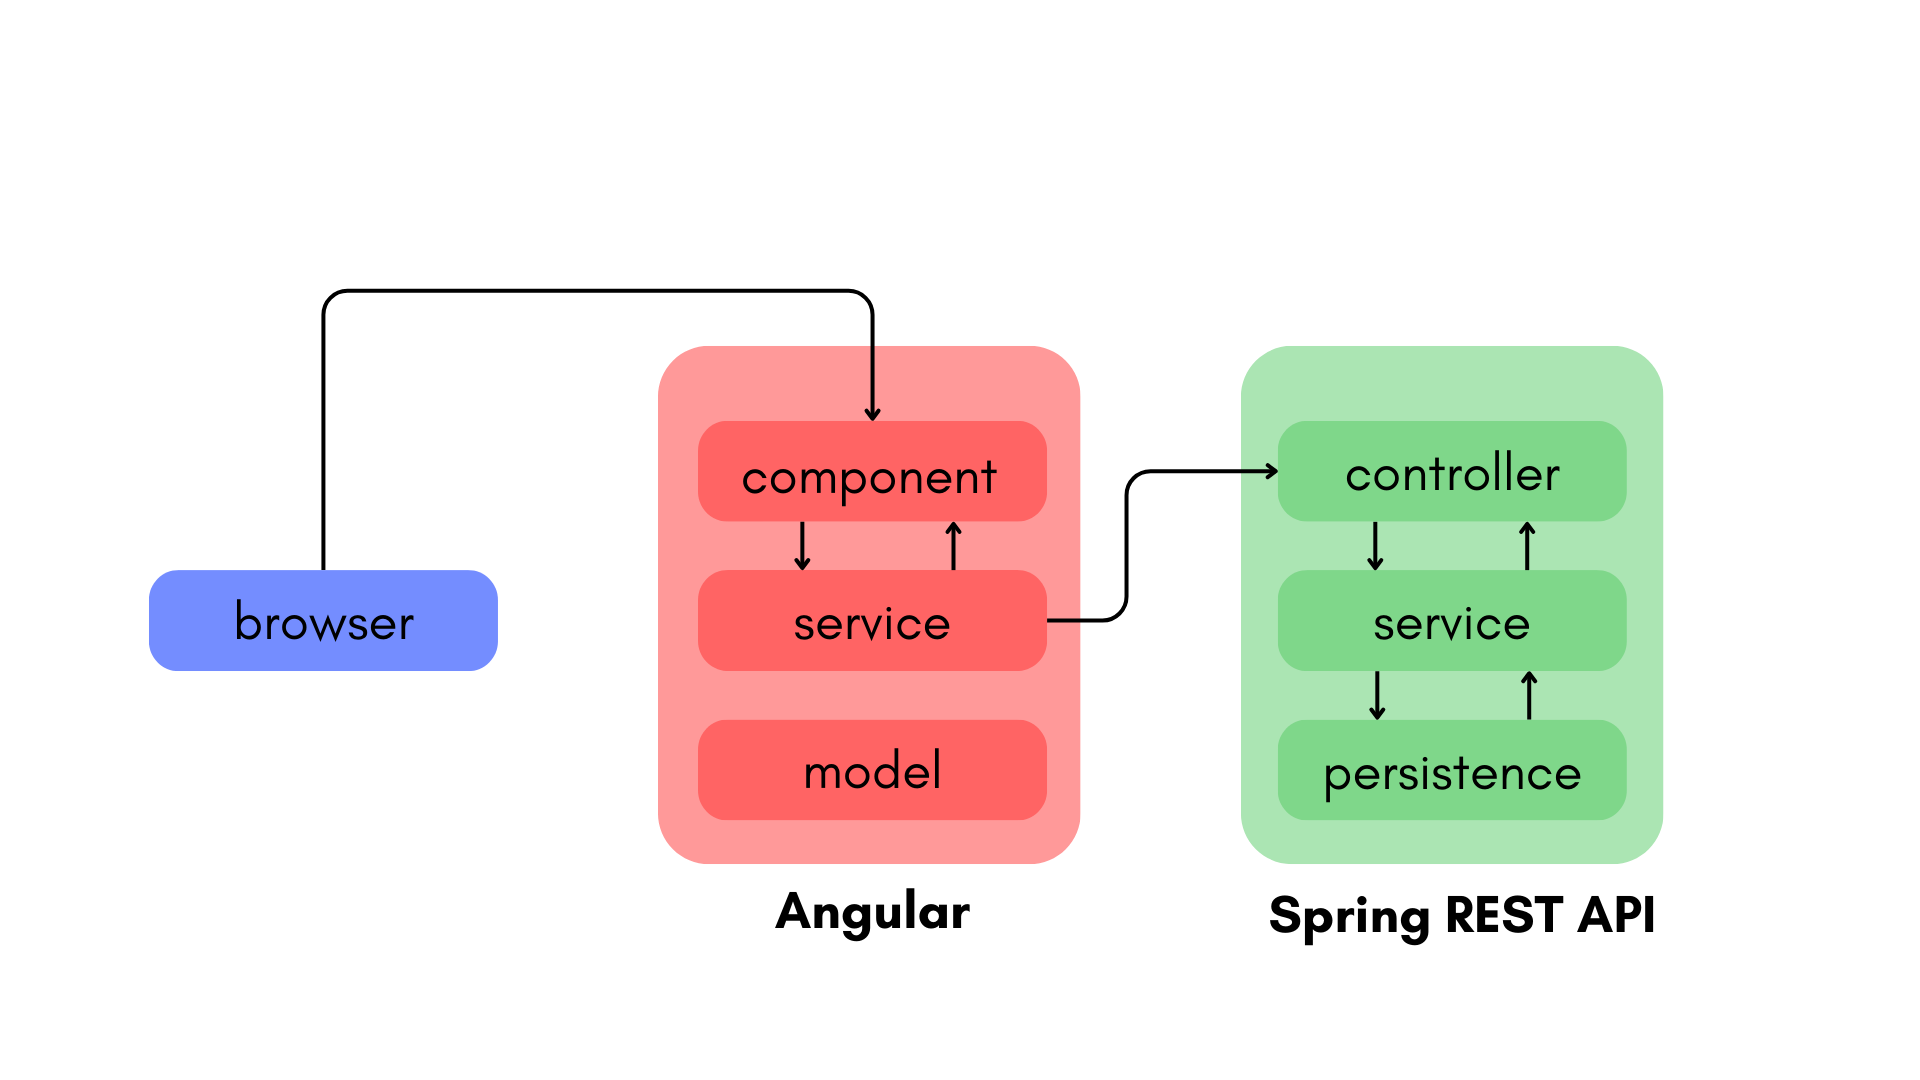
\includegraphics[width=\textwidth]{images/angular_spring_diagram.png}
\end{tcolorbox}
\section{Importance du Flux entre les Parties}

L’ordre de développement est essentiel pour éviter des erreurs et des inefficacités :
\begin{enumerate}
    \item \textbf{Module :} Structure la fonctionnalité et facilite son intégration.
    \item \textbf{Service :} Gère les données et les processus liés à la fonctionnalité.
    \item \textbf{Composant :} Présente les données à l’utilisateur et capture ses actions.
\end{enumerate}

Ce flux garantit une architecture propre, avec des responsabilités bien définies et un code facile à maintenir.
\section*{Modules dans Angular : Structure et Fonctionnement}

Dans Angular, les \textbf{modules} jouent un rôle clé dans l'organisation de l'application. Ils permettent de regrouper des composants, des services, des directives, des pipes et d'autres modules afin de rendre l'application modulaire, réutilisable et facilement maintenable. Chaque module est associé à un fichier TypeScript qui sert de point d'entrée pour le module, le plus important étant \textbf{AppModule}, le module principal.

\subsection*{1. AppModule : Le Point d'Entrée de l'Application}

Le \textbf{AppModule} est le module de base de toute application Angular. C'est le module qui est chargé lors du démarrage de l'application. Il regroupe tous les autres modules nécessaires au bon fonctionnement de l'application.

\textbf{Déclaration d'AppModule :}  
AppModule est un module Angular classique qui contient les informations essentielles pour démarrer l'application, comme la déclaration des composants, l'importation des modules nécessaires, les services, et l’injection des dépendances.

\textbf{Exemple :}  
\begin{lstlisting}[language=TypeScript, caption={Using a service in a component}, label={lst:typescript-service-usage}]

import { NgModule } from '@angular/core';
import { BrowserModule } from '@angular/platform-browser';
import { AppComponent } from './app.component';

@NgModule({
  declarations: [  // Déclare tous les composants utilisés par ce module
    AppComponent
  ],
  imports: [  // Importation d'autres modules nécessaires
    BrowserModule
  ],
  providers: [],  // Déclaration des services
  bootstrap: [AppComponent]  // Composant qui démarre l'application
})
export class AppModule { }
\end{lstlisting}

\subsection*{2. Structure des Modules Angular}

Un module Angular est défini à l’aide du décorateur \texttt{@NgModule}, qui prend un objet avec plusieurs propriétés clés. Ces propriétés permettent de configurer le module en fonction des besoins spécifiques de l'application.

\subsubsection*{2.1 Declarations}
La propriété \texttt{declarations} regroupe tous les \textbf{composants}, \textbf{directives} et \textbf{pipes} utilisés dans le module. Chaque composant, directive ou pipe doit être déclaré dans un module pour qu’il soit reconnu et utilisé.

\begin{itemize}
    \item \textbf{Composants :} Représentent l’interface utilisateur.
    \item \textbf{Directives :} Modifient l’apparence ou le comportement d’un élément du DOM.
    \item \textbf{Pipes :} Permettent de transformer les données affichées à l'utilisateur.
\end{itemize}

\textbf{Exemple :}  
\begin{verbatim}
@NgModule({
  declarations: [
    AppComponent,
    HeaderComponent,
    FooterComponent
  ]
})
\end{verbatim}

\subsubsection*{2.2 Imports}
La propriété \texttt{imports} contient une liste de \textbf{modules externes} que ce module utilise. Cela permet de regrouper les fonctionnalités d’autres modules, par exemple, le module de routage ou le module de formulaires.

\begin{itemize}
    \item Par exemple, vous pouvez importer des modules comme \texttt{FormsModule}, \texttt{HttpClientModule}, \texttt{RouterModule}, etc.
\end{itemize}

\textbf{Exemple :}  
\begin{lstlisting}[language=TypeScript, caption={Using a service in a component}, label={lst:typescript-service-usage}]

import { FormsModule } from '@angular/forms';
import { RouterModule } from '@angular/router';

@NgModule({
  imports: [
    BrowserModule,  // Module de base pour le navigateur
    FormsModule,    // Module pour les formulaires
    RouterModule    // Module pour la gestion du routage
  ]
})
\end{lstlisting}

\subsubsection*{2.3 Providers}
La propriété \texttt{providers} permet de déclarer les \textbf{services} que vous souhaitez injecter dans l'application. Cela permet à Angular d’injecter ces services dans les composants et autres services via l’injection de dépendances.

\begin{itemize}
    \item Les services peuvent être fournis à l’échelle du module ou de l’application entière en utilisant des \texttt{providers} dans \texttt{@NgModule}.
\end{itemize}

\textbf{Exemple :}  
\begin{lstlisting}[language=TypeScript, caption={Using a service in a component}, label={lst:typescript-service-usage}]

import { ProductService } from './product.service';

@NgModule({
  providers: [
    ProductService  // Déclaration du service à utiliser dans l'application
  ]
})
\end{lstlisting}

\subsubsection*{2.4 Bootstrap}
La propriété \texttt{bootstrap} permet de spécifier le ou les \textbf{composants principaux} qui démarrent l'application. C’est ici que vous déclarez le composant racine de votre application, généralement \texttt{AppComponent}.

\begin{itemize}
    \item \texttt{AppComponent} est le composant qui sera utilisé pour initialiser l’interface utilisateur de l'application.
\end{itemize}

\textbf{Exemple :}  
\begin{verbatim}
@NgModule({
  bootstrap: [AppComponent]  // Définition du composant qui démarre l'application
})
\end{verbatim}

\subsection*{3. Exemple Complet d’un Module Angular}

Voici un exemple d'un module complet avec les différentes parties que nous avons abordées :

\begin{lstlisting}[language=TypeScript, caption={Using a service in a component}, label={lst:typescript-service-usage}]

import { NgModule } from '@angular/core';
import { BrowserModule } from '@angular/platform-browser';
import { FormsModule } from '@angular/forms';  // Pour les formulaires
import { RouterModule } from '@angular/router';  // Pour le routage

import { AppComponent } from './app.component';
import { HeaderComponent } from './header/header.component';
import { FooterComponent } from './footer/footer.component';
import { ProductService } from './services/product.service';

@NgModule({
  declarations: [
    AppComponent,  // Composant principal
    HeaderComponent,  // Composant de l'en-tête
    FooterComponent   // Composant du pied de page
  ],
  imports: [
    BrowserModule,  // Module de base pour le navigateur
    FormsModule,    // Module pour les formulaires
    RouterModule    // Module pour la gestion du routage
  ],
  providers: [
    ProductService  // Service pour gérer les produits
  ],
  bootstrap: [AppComponent]  // Composant principal qui démarre l'application
})
export class AppModule { }
\end{lstlisting}

\subsection*{4. Rôle de \texttt{AppModule} dans le Flux d'Information}

Le \textbf{AppModule} sert de point d’entrée et de point de coordination pour toutes les fonctionnalités de l’application.  
\begin{itemize}
    \item Dès que l'application démarre, Angular charge le \textbf{AppModule}.
    \item Il \textbf{déclare} les composants, \textbf{importe} les autres modules nécessaires (comme ceux pour les formulaires, les services HTTP, etc.), \textbf{déclare les services} qu’il fournit à l’application et \textbf{initialise} le \textbf{composant principal (AppComponent)}.
\end{itemize}

\subsection*{5. Conclusion}

L’architecture d’un module Angular permet de structurer et d’organiser les fonctionnalités de manière efficace et maintenable. La structure d’un module — \textbf{Declarations}, \textbf{Imports}, \textbf{Providers}, et \textbf{Bootstrap} — est essentielle pour définir comment les différentes parties de l’application interagiront et seront accessibles à travers les autres modules et composants.

\textbf{Conseil pratique :} Commencez par définir vos modules pour organiser l'application en fonctionnalités indépendantes. Ensuite, ajoutez les composants et services nécessaires et assurez-vous qu’ils sont correctement injectés dans les modules.


Dans Angular, les \textbf{composants} sont les éléments fondamentaux pour construire l'interface utilisateur (UI). Chaque composant représente une \textbf{partie spécifique de l'UI}, comme un bouton, une page, ou un formulaire. Les composants permettent de diviser l'interface utilisateur en éléments modulaires, réutilisables et faciles à maintenir.

Chaque composant dans Angular est associé à un \textbf{décorateur \@Component} qui fournit des métadonnées sur le composant, y compris la structure HTML, le style CSS et le comportement en TypeScript.

\section*{1. Le Rôle d’un Composant dans Angular}

Un \textbf{composant} sert à :
\begin{itemize}
  \item \textbf{Gérer l’interface utilisateur} d’une section de l’application (ex : un formulaire, une barre de navigation).
  \item \textbf{Capturer les interactions} de l'utilisateur (ex : clics, saisie dans des champs de formulaire).
  \item \textbf{Communiquer avec d’autres composants ou services} pour récupérer ou manipuler des données.
\end{itemize}

En résumé, les composants sont les briques de base de l’application Angular, et leur rôle principal est de lier l'affichage et la logique métier.

\section*{2. Utilisation du Décorateur \@Component}

Le décorateur \@Component est une fonction qui permet de configurer un composant Angular. Il est utilisé pour définir les métadonnées du composant, telles que le modèle HTML, le style CSS, et le comportement TypeScript. Il permet également de connecter un composant à un module spécifique.

Le décorateur \@Component prend un objet contenant plusieurs propriétés essentielles :
\begin{itemize}
  \item \textbf{selector} : Déclare le nom de l’élément HTML personnalisé qui représente ce composant dans le DOM.
  \item \textbf{templateUrl} ou \textbf{template} : Lien vers le fichier HTML ou code HTML inline utilisé pour le modèle du composant.
  \item \textbf{styleUrls} ou \textbf{styles} : Lien vers le fichier CSS ou code CSS inline utilisé pour le style du composant.
  \item \textbf{providers} : Déclare les services utilisés dans ce composant.
\end{itemize}

\textbf{Exemple de décorateur \@Component :}
\begin{lstlisting}[language=TypeScript, caption={Using a service in a component}, label={lst:typescript-service-usage}]

import { Component } from '@angular/core';

@Component({
  selector: 'app-header',  // Déclare un élément HTML personnalisé
  templateUrl: './header.component.html',  // Lien vers le modèle HTML
  styleUrls: ['./header.component.css']   // Lien vers le fichier CSS du composant
})
export class HeaderComponent {
  title: string = "Bienvenue sur notre site";
}
\end{lstlisting}

\section*{3. Structure d’un Composant}

Un composant Angular est composé de trois fichiers principaux :
\begin{enumerate}
  \item \textbf{HTML (Template)} : Définit l’interface utilisateur du composant.
  \item \textbf{CSS (Styles)} : Définit les styles associés à l’interface du composant.
  \item \textbf{TypeScript (Classe)} : Contient la logique métier du composant, gère les données et les événements utilisateur.
\end{enumerate}

\subsection*{3.1 Le Fichier HTML (Template)}

Le fichier HTML définit la structure de l'interface utilisateur. Il peut contenir des balises HTML de base ainsi que des directives Angular pour lier les données et gérer les événements.

\textbf{Exemple de template HTML :}
\begin{verbatim}
<div class="header">
  <h1>{{ title }}</h1>
  <button (click)="onClick()">Cliquez ici</button>
</div>
\end{verbatim}
- \texttt{{\{ title \}}} : C’est une \textbf{liaison de données} (data binding) qui affiche la valeur de la propriété \texttt{title} du composant.
- \texttt{(click)="onClick()"} : Cette syntaxe est un \textbf{binding d'événements} qui lie un événement du DOM (comme un clic) à une méthode TypeScript (ici \texttt{onClick()}). 

\subsection*{3.2 Le Fichier CSS (Styles)}

Le fichier CSS contient les styles spécifiques au composant. Angular utilise un système d'encapsulation de styles pour éviter que les styles d’un composant n'affectent d'autres composants.

\textbf{Exemple de fichier CSS :}
\begin{verbatim}
.header {
  background-color: #4CAF50;
  color: white;
  padding: 10px;
}
\end{verbatim}

\subsection*{3.3 Le Fichier TypeScript (Classe)}

Le fichier TypeScript contient la \textbf{classe du composant} qui gère les propriétés et les méthodes de ce composant. C’est ici que vous définissez la logique métier, l’état interne du composant, et les comportements en réponse aux interactions utilisateur.

\textbf{Exemple de classe TypeScript :}
\begin{lstlisting}[language=TypeScript, caption={Using a service in a component}, label={lst:typescript-service-usage}]

import { Component } from '@angular/core';

@Component({
  selector: 'app-header',
  templateUrl: './header.component.html',
  styleUrls: ['./header.component.css']
})
export class HeaderComponent {
  title: string = "Bienvenue sur notre site";

  onClick() {
    console.log("Le bouton a été cliqué!");
  }
}
\end{lstlisting}
- La \textbf{propriété \texttt{title}} contient des données que l’on veut afficher dans le template HTML.
- La méthode \textbf{\texttt{onClick()}} gère l'événement de clic sur le bouton.

\section*{4. Flux de Données et Interactions dans un Composant}

Les composants interagissent principalement avec :
\begin{itemize}
  \item \textbf{Les propriétés et méthodes} dans la classe TypeScript.
  \item \textbf{Le template HTML}, via des liaisons de données.
  \item \textbf{Les services} pour manipuler les données ou faire des appels API.
\end{itemize}

\subsection*{4.1 Liaison de données (Data Binding)}

Angular propose plusieurs types de liaison de données :
\begin{itemize}
  \item \textbf{Liaison unidirectionnelle (One-way Binding)} : De la classe vers le template (ou inversement).
    \begin{itemize}
      \item \texttt{{\{ value \}}} : Interpolation pour afficher des valeurs dans le template.
      \item \texttt{[property]="value"} : Liaison des propriétés d’un élément HTML avec la propriété d’un composant.
      \item \texttt{(event)="handler()"} : Lier un événement DOM à une méthode dans la classe.
    \end{itemize}
  \item \textbf{Liaison bidirectionnelle (Two-way Binding)} : Utilisation de \texttt{[(ngModel)]} pour lier les données dans les formulaires.
\end{itemize}

\textbf{Exemple de liaison bidirectionnelle :}
\begin{verbatim}
<input [(ngModel)]="username">
<p>Bienvenue, {{ username }}!</p>
\end{verbatim}

\section*{5. Exemple Complet d’un Composant}

Voici un exemple complet d’un composant :

\subsection*{HTML (Template) :}
\begin{lstlisting}[language=HTML, caption={HTML example of a login form}, label={lst:login-form}]
<div class="login-form">
  <h2>{{ title }}</h2>
  <input [(ngModel)]="username" placeholder="Entrez votre nom">
  <button (click)="onSubmit()">Se connecter</button>
</div>
\end{lstlisting}

\subsection*{CSS (Styles) :}
\begin{lstlisting}[language=CSS, caption={CSS styling for login form}, label={lst:css-login-form}]
.login-form {
  margin: 20px;
  padding: 15px;
  border: 1px solid #ccc;
}
input {
  padding: 5px;
  margin-bottom: 10px;
}
button {
  background-color: #4CAF50;
  color: white;
  padding: 10px 20px;
}
\end{lstlisting}


\subsection*{TypeScript (Classe) :}
\begin{lstlisting}[language=TypeScript, caption={TypeScript class for login functionality}, label={lst:typescript-login}]
import { Component } from '@angular/core';

@Component({
  selector: 'app-login',
  templateUrl: './login.component.html',
  styleUrls: ['./login.component.css']
})
export class LoginComponent {
  title: string = 'Connexion';
  username: string = '';

  onSubmit() {
    console.log(`Nom d'utilisateur: ${this.username}`);
  }
}
\end{lstlisting}


\section*{6. Conclusion}

Les \textbf{composants} sont les éléments clés pour construire l'interface utilisateur dans Angular. Chaque composant est constitué de trois parties essentielles :
\begin{itemize}
  \item \textbf{HTML} pour la structure de l'interface,
  \item \textbf{CSS} pour le style,
  \item \textbf{TypeScript} pour la logique et la gestion des données.
\end{itemize}

Le décorateur \@Component permet de lier ces trois parties et de définir comment le composant interagira avec d’autres composants ou services, tout en permettant une gestion efficace des événements et des données.

\textbf{Conseil pratique} : Lors de la création d’un composant, commencez toujours par définir le modèle HTML (structure), puis implémentez la logique nécessaire dans la classe TypeScript, et enfin, ajoutez les styles pour que l’interface soit propre et intuitive.

\section{Liaison de Données : Unidirectionnelle et Bidirectionnelle}


Dans Angular, le \textbf{template} d’un composant est responsable de l’interface utilisateur, tandis que la \textbf{liaison de données} permet de relier le modèle de données (les propriétés et méthodes de la classe du composant) au DOM (le modèle de l'interface utilisateur). 

Il existe plusieurs types de liaison de données qui permettent à Angular de synchroniser les données entre le composant et la vue de manière efficace.

\section{Liaison de Données : Unidirectionnelle et Bidirectionnelle}

\subsection{Liaison unidirectionnelle (One-way Binding)}

Dans la liaison unidirectionnelle, les données circulent dans une seule direction : soit du composant vers la vue (affichage), soit de la vue vers le composant (interactions utilisateur).
\begin{tcolorbox}[colframe=black!70, colback=white, title=Figure 5: Liaison unidirectionnelle, fonttitle=\bfseries]
\centering
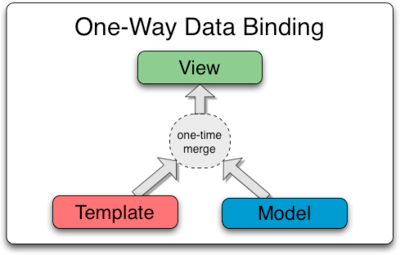
\includegraphics[width=\textwidth]{images/angularjs-one-way-data-binding.png}
\end{tcolorbox}
\subsubsection{Interpolation (du composant vers la vue)}

Permet de lier une valeur de la classe TypeScript à une section de l'HTML.
\begin{verbatim}
<p>{{ title }}</p>
\end{verbatim}
Dans cet exemple, le contenu de \texttt{title} dans la classe du composant sera affiché dans le \texttt{<p>}.

\subsubsection{Liaison de propriétés (du composant vers la vue)}

Permet de lier une propriété d'un élément HTML à une propriété du composant.
\begin{verbatim}
<img [src]="imageUrl" alt="Image dynamique">
\end{verbatim}
Ici, l'attribut \texttt{src} de l'image est lié à la propriété \texttt{imageUrl} du composant.

\subsubsection{Liaison d'événements (de la vue vers le composant)}

Permet de lier un événement DOM (comme un clic) à une méthode dans la classe du composant.
\begin{verbatim}
<button (click)="onClick()">Cliquez ici</button>
\end{verbatim}
L'événement \texttt{click} déclenche la méthode \texttt{onClick()} du composant lorsqu'on clique sur le bouton.

\subsection{Liaison bidirectionnelle (Two-way Binding)}

La liaison bidirectionnelle permet de lier une donnée dans le modèle et la vue, de sorte que toute modification dans l’un des deux se reflète instantanément dans l’autre.
\begin{tcolorbox}[colframe=black!70, colback=white, title=Figure 6: Liaison bidirectionnelle, fonttitle=\bfseries]
\centering
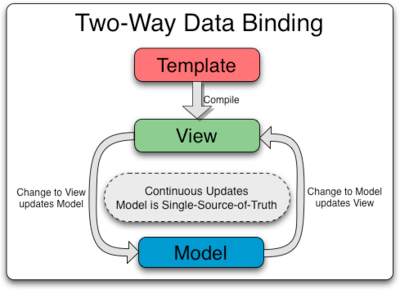
\includegraphics[width=\textwidth]{images/angularjs-two-way-data-binding.png}
\end{tcolorbox}
Angular implémente cela principalement avec la directive \texttt{ngModel}, qui permet de lier un champ de formulaire avec une propriété de la classe du composant.

\begin{verbatim}
<input [(ngModel)]="username">
<p>Nom d'utilisateur : {{ username }}</p>
\end{verbatim}

Dans cet exemple, la valeur de \texttt{username} est liée à l'input. Si l'utilisateur tape quelque chose, \texttt{username} est mis à jour automatiquement, et si la propriété \texttt{username} change dans le composant, l'input sera également mis à jour.

\section{Utilisation de Directives Angular}

Les \textbf{directives} sont des classes qui modifient le comportement des éléments du DOM. Elles sont utilisées pour créer des comportements réutilisables dans l'interface utilisateur.

\subsection{Directives structurelles}

Les directives structurelles modifient la structure du DOM en ajoutant ou en supprimant des éléments. Elles sont généralement utilisées pour \textbf{contrôler la visibilité} ou la \textbf{répétition d'éléments}.

\subsubsection{*ngIf}

Cette directive permet de conditionner l’affichage d’un élément du DOM en fonction d’une expression. Si l'expression est vraie, l'élément est affiché ; sinon, il est supprimé du DOM.
\begin{verbatim}
<div *ngIf="isVisible">Ce contenu est visible si isVisible est true.</div>
\end{verbatim}

\subsubsection{*ngFor}

Cette directive permet de répéter un élément pour chaque élément d’une collection.
\begin{verbatim}
<ul>
  <li *ngFor="let item of items">{{ item }}</li>
</ul>
\end{verbatim}

\subsection{Directives attributs}

Les directives attributs modifient l’apparence ou le comportement d’un élément sans changer sa structure.

\subsubsection{ngClass}

Cette directive permet d’ajouter ou de retirer des classes CSS d’un élément en fonction des conditions spécifiées dans l’expression.
\begin{verbatim}
<div [ngClass]="{'highlight': isHighlighted}">Ce texte est mis en surbrillance si isHighlighted est true.</div>
\end{verbatim}

\subsubsection{ngStyle}

Cette directive permet d’ajouter ou de modifier dynamiquement les styles d’un élément.
\begin{verbatim}
<div [ngStyle]="{'color': color, 'font-size': fontSize + 'px'}">Ce texte a des styles dynamiques.</div>
\end{verbatim}

\section{Services et Injection de Dépendances}

Les \textbf{services} jouent un rôle essentiel dans Angular pour gérer les \textbf{logiques métiers}, accéder aux données et effectuer des traitements externes. Ils sont utilisés pour fournir des fonctionnalités réutilisables dans toute l’application. Les services sont généralement utilisés pour communiquer avec des API, manipuler des données ou stocker des informations.
\begin{tcolorbox}[colframe=black!70, colback=white, title=Figure 7: Services et Injection de D´ependances, fonttitle=\bfseries]
\centering
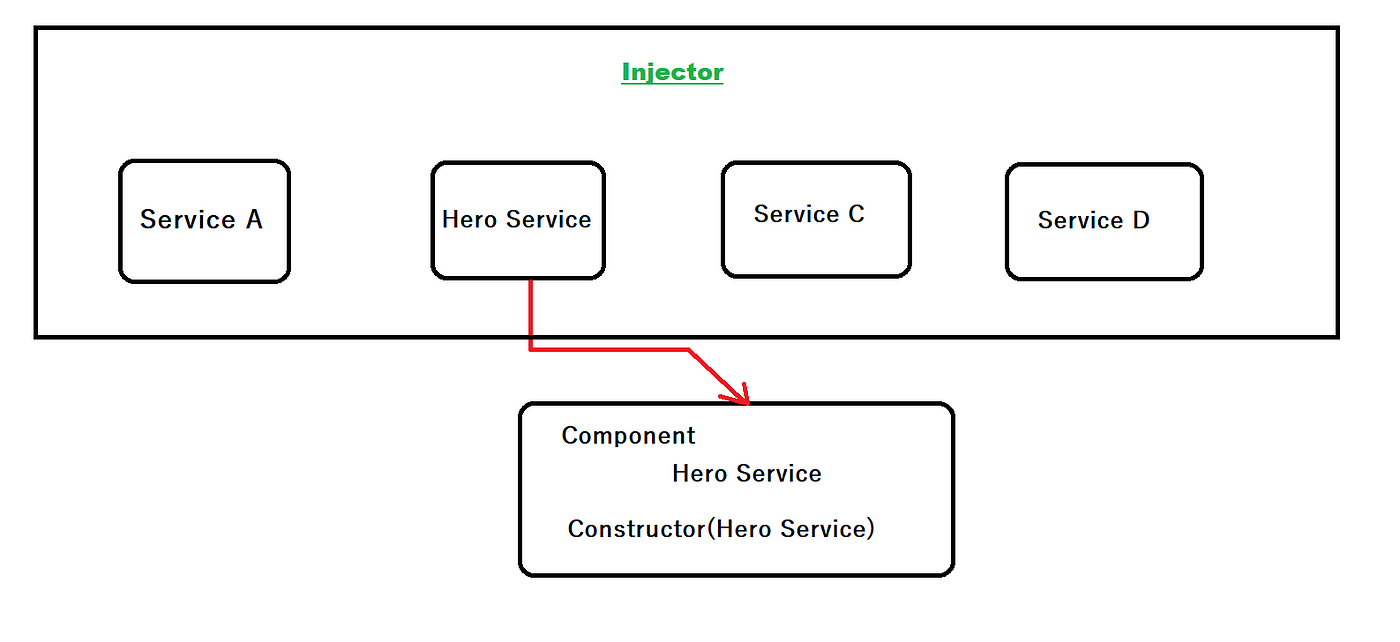
\includegraphics[width=\textwidth]{images/0_R0nqYsF51ACGiI_K.png}
\end{tcolorbox}

\subsection{Rôle des Services dans Angular}

Un service est une \textbf{classe} qui encapsule une logique ou un comportement spécifique. Les services sont souvent utilisés pour :
\begin{itemize}
  \item \textbf{Partager des données entre composants} : Un service peut stocker des données partagées et permettre aux composants de les lire ou de les modifier.
  \item \textbf{Communiquer avec des API} : Un service peut être utilisé pour gérer les appels HTTP et récupérer des données depuis un serveur.
  \item \textbf{Gérer l’état de l’application} : Un service peut contenir des informations qui doivent être accessibles à plusieurs composants, comme l'état d'authentification d'un utilisateur ou les paramètres de l'application.
\end{itemize}

\subsection{Injection de Dépendances avec \texttt{@Injectable}}

L'\textbf{injection de dépendances} (DI) est un concept fondamental dans Angular qui permet d’injecter des objets (comme des services) dans des composants ou d'autres services. Cela facilite la gestion des dépendances sans que les classes aient besoin de créer ces objets elles-mêmes.

\subsubsection{\texttt{@Injectable()}}

C’est un décorateur qui marque une classe comme un \textbf{service injectable}. Il indique à Angular que cette classe peut être \textbf{injectée} dans d’autres composants ou services.

Voici un exemple simple d'un service avec l'injection de dépendances :

\begin{lstlisting}[language=TypeScript, caption={TypeScript service example}, label={lst:typescript-service}]
import { Injectable } from '@angular/core';

@Injectable({
  providedIn: 'root' // This indicates that the service is available at the application level
})
export class DataService {
  private data: string[] = [];

  constructor() { }

  getData(): string[] {
    return this.data;
  }

  addData(newData: string): void {
    this.data.push(newData);
  }
}
\end{lstlisting}

\subsection{Utilisation du service dans un composant}

Dans le composant, vous \textbf{injectez} le service pour y accéder :

\begin{lstlisting}[language=TypeScript, caption={Using a service in a component}, label={lst:typescript-service-usage}]
import { Component } from '@angular/core';
import { DataService } from './data.service';  // Import the service

@Component({
  selector: 'app-data-list',
  templateUrl: './data-list.component.html',
  styleUrls: ['./data-list.component.css']
})
export class DataListComponent {
  data: string[] = [];

  constructor(private dataService: DataService) { } // Inject the service

  ngOnInit(): void {
    this.data = this.dataService.getData();
  }

  addData(newData: string): void {
    this.dataService.addData(newData);
  }
}
\end{lstlisting}

Dans cet exemple, \texttt{DataService} est injecté dans \texttt{DataListComponent} via le constructeur. Vous pouvez appeler les méthodes du service pour récupérer ou manipuler les données. 

\section{Conclusion}

\begin{itemize}
  \item \textbf{Templates et Liaison de Données} : La liaison de données permet de synchroniser le modèle (données) avec la vue (interface utilisateur). Les liaisons unidirectionnelles et bidirectionnelles facilitent l’interaction entre le modèle et la vue.
  \item \textbf{Directives Angular} : Angular propose des directives puissantes comme \texttt{*ngIf}, \texttt{*ngFor}, \texttt{ngClass} et \texttt{ngStyle}, qui permettent de modifier la structure ou les styles des éléments du DOM de manière déclarative.
  \item \textbf{Services et Injection de Dépendances} : Les services encapsulent la logique métier et les données partagées. Grâce à l'injection de dépendances, les services peuvent être facilement injectés dans les composants, permettant de maintenir un code modulaire et réutilisable.
\end{itemize}

Ces concepts fondamentaux d'Angular sont essentiels pour développer des applications robustes et bien structurées.


\section*{Routage dans Angular}

Le \textbf{routage} permet de naviguer entre différentes vues de l'application. Dans Angular, le routage est configuré en utilisant le module \texttt{RouterModule} et permet de lier des composants à des URL spécifiques.

\subsection*{1. Configuration des Routes dans \texttt{app-routing.module.ts}}

Dans Angular, les routes sont définies dans un fichier de module appelé \texttt{app-routing.module.ts}. Ce module importe le \texttt{RouterModule} et utilise la méthode \texttt{RouterModule.forRoot(routes)} pour configurer les différentes routes.

Voici un exemple de configuration de routes :
\begin{lstlisting}[language=TypeScript, caption={Using a service in a component}, label={lst:typescript-service-usage}]

import { NgModule } from '@angular/core';
import { RouterModule, Routes } from '@angular/router';
import { HomeComponent } from './home/home.component';
import { AboutComponent } from './about/about.component';

const routes: Routes = [
  { path: '', component: HomeComponent },
  { path: 'about', component: AboutComponent }
];

@NgModule({
  imports: [RouterModule.forRoot(routes)],
  exports: [RouterModule]
})
export class AppRoutingModule { }
\end{lstlisting}

Dans cet exemple :
- La route par défaut (\texttt{path: ''}) charge le \texttt{HomeComponent}.
- La route \texttt{/about} charge le \texttt{AboutComponent}.

\subsection*{2. Navigation entre Composants et Gestion des Paramètres de Route}

Pour naviguer entre les composants, on utilise la directive \texttt{routerLink} dans le template, qui permet de lier une URL à un élément.

Exemple :
\begin{lstlisting}[language=TypeScript, caption={Using a service in a component}, label={lst:typescript-service-usage}]

<a routerLink="/about">À propos</a>
\end{lstlisting}

\textbf{Gestion des paramètres de route} :
Parfois, on doit récupérer des paramètres dans l'URL. Cela peut être fait en utilisant \texttt{ActivatedRoute} dans le composant cible.

Exemple :
\begin{lstlisting}[language=TypeScript, caption={Using a service in a component}, label={lst:typescript-service-usage}]

import { ActivatedRoute } from '@angular/router';

@Component({
  selector: 'app-about',
  templateUrl: './about.component.html',
  styleUrls: ['./about.component.css']
})
export class AboutComponent implements OnInit {

  constructor(private route: ActivatedRoute) { }

  ngOnInit(): void {
    this.route.params.subscribe(params => {
      const id = params['id']; // Récupère un paramètre 'id' de l'URL
      console.log(id);
    });
  }
}
\end{lstlisting}

\section*{Formulaires dans Angular}

Les formulaires permettent de collecter des informations de l'utilisateur. Angular propose deux approches principales pour gérer les formulaires : \textbf{les formulaires basés sur des templates} et \textbf{les formulaires réactifs}.

\subsection*{1. Formulaires Basés sur des Templates}

Dans cette approche, le formulaire et ses validations sont principalement définis dans le template HTML.

Exemple :
\begin{lstlisting}[language=TypeScript, caption={Using a service in a component}, label={lst:typescript-service-usage}]

<form #myForm="ngForm" (ngSubmit)="onSubmit(myForm)">
  <input name="username" ngModel required />
  <button type="submit" [disabled]="!myForm.valid">Submit</button>
</form>
\end{lstlisting}

Dans ce cas, \texttt{ngForm} est une directive qui crée un objet de formulaire, et \texttt{ngModel} lie les champs à la classe du composant.

\subsection*{2. Formulaires Réactifs}

Les formulaires réactifs sont plus puissants et flexibles. Ils sont définis dans le composant et sont utilisés pour créer des formulaires complexes avec des validations avancées.

Exemple :
\begin{lstlisting}[language=TypeScript, caption={Using a service in a component}, label={lst:typescript-service-usage}]

import { Component, OnInit } from '@angular/core';
import { FormBuilder, FormGroup, Validators } from '@angular/forms';

@Component({
  selector: 'app-login',
  templateUrl: './login.component.html',
  styleUrls: ['./login.component.css']
})
export class LoginComponent implements OnInit {

  loginForm: FormGroup;

  constructor(private fb: FormBuilder) { }

  ngOnInit(): void {
    this.loginForm = this.fb.group({
      username: ['', Validators.required],
      password: ['', [Validators.required, Validators.minLength(6)]]
    });
  }

  onSubmit(): void {
    if (this.loginForm.valid) {
      console.log(this.loginForm.value);
    }
  }
}
\end{lstlisting}

Ici, nous utilisons \texttt{FormBuilder} pour créer un formulaire réactif et y appliquer des validations.

\section*{Pipes dans Angular}

Les \textbf{pipes} sont utilisés pour transformer les données affichées dans l'interface utilisateur. Ils sont souvent utilisés pour formater les valeurs, comme les dates ou les devises.

\subsection*{1. Pipes Intégrés}

Angular propose plusieurs pipes intégrés pour effectuer des transformations courantes :
- \texttt{date} : Formate une date.
    \begin{verbatim}
    <p>{{ currentDate | date:'shortDate' }}</p>
    \end{verbatim}
  
- \texttt{currency} : Affiche une valeur sous forme de devise.
    \begin{verbatim}
    <p>{{ amount | currency:'EUR' }}</p>
    \end{verbatim}

\subsection*{2. Création de Pipes Personnalisés}

Il est possible de créer des pipes personnalisés pour effectuer des transformations spécifiques aux besoins de l’application.

Exemple :
\begin{lstlisting}[language=TypeScript, caption={Using a service in a component}, label={lst:typescript-service-usage}]

import { Pipe, PipeTransform } from '@angular/core';

@Pipe({
  name: 'reverse'
})
export class ReversePipe implements PipeTransform {
  transform(value: string): string {
    return value.split('').reverse().join('');
  }
}
\end{lstlisting}

Dans le template :
\begin{verbatim}
<p>{{ 'Hello' | reverse }}</p> <!-- Affiche 'olleH' -->
\end{verbatim}

\section*{Gestion des Données et HTTP}

Angular permet d'effectuer des requêtes HTTP en utilisant le module \texttt{HttpClientModule}, ce qui facilite la consommation d'APIs externes.

\subsection*{1. Utilisation de \texttt{HttpClientModule}}

Pour consommer des API REST, vous devez d'abord importer le module \texttt{HttpClientModule} dans le fichier \texttt{app.module.ts} :

\begin{lstlisting}[language=TypeScript, caption={Using a service in a component}, label={lst:typescript-service-usage}]

import { HttpClientModule } from '@angular/common/http';

@NgModule({
  imports: [HttpClientModule],
  // autres configurations...
})
export class AppModule { }
\end{lstlisting}

Ensuite, dans votre service ou composant, vous utilisez \texttt{HttpClient} pour faire des requêtes HTTP.

Exemple d'appel GET :
\begin{lstlisting}[language=TypeScript, caption={Using a service in a component}, label={lst:typescript-service-usage}]

import { HttpClient } from '@angular/common/http';

@Component({
  selector: 'app-data',
  templateUrl: './data.component.html',
  styleUrls: ['./data.component.css']
})
export class DataComponent {

  constructor(private http: HttpClient) {}

  fetchData(): void {
    this.http.get('https://api.example.com/data').subscribe(data => {
      console.log(data);
    });
  }
}
\end{lstlisting}

\subsection*{2. Consommation d’API REST et Gestion des Erreurs}

Lors de la consommation d'APIs, il est important de gérer les erreurs avec \texttt{catchError} et de traiter les réponses asynchrones.

Exemple de gestion des erreurs :
\begin{lstlisting}[language=TypeScript, caption={Using a service in a component}, label={lst:typescript-service-usage}]

import { catchError } from 'rxjs/operators';
import { throwError } from 'rxjs';

this.http.get('https://api.example.com/data')
  .pipe(catchError(error => {
    console.error('Error occurred:', error);
    return throwError(error);
  }))
  .subscribe(data => {
    console.log(data);
  });
\end{lstlisting}

\section*{RxJS et Observables}

Les \textbf{Observables} sont une partie centrale d'Angular et sont utilisés pour gérer les flux de données asynchrones, comme les requêtes HTTP, les événements utilisateurs, ou les modifications de données.

\subsection*{1. Introduction à RxJS}

RxJS (Reactive Extensions for JavaScript) est une bibliothèque pour composer des programmes asynchrones et basés sur des événements en utilisant des observables.

Un \textbf{observable} est un flux de données qui peut être observé. Un \textbf{subscriber} peut s’abonner à cet observable pour recevoir les valeurs émises.

Exemple de base avec un observable :
\begin{lstlisting}[language=TypeScript, caption={Using a service in a component}, label={lst:typescript-service-usage}]

import { Observable } from 'rxjs';

const observable = new Observable(subscriber => {
  subscriber.next('Hello');
  subscriber.complete();
});

observable.subscribe(value => console.log(value));  // Affiche 'Hello'
\end{lstlisting}

\subsection*{2. Utilisation des Observables pour Gérer les Flux de Données}

Les observables permettent de gérer les flux de données de manière réactive, par exemple, pour manipuler les données reçues d’une API, les événements utilisateurs, etc.

Exemple avec une requête HTTP :
\begin{lstlisting}[language=TypeScript, caption={Using a service in a component}, label={lst:typescript-service-usage}]

this.http.get('https://api.example.com/data')
  .subscribe(data => {
    this.data = data;
  });
\end{lstlisting}

\section*{Lazy Loading et Optimisation}

Le \textbf{Lazy Loading} permet de charger les modules Angular de manière différée, réduisant ainsi le temps de chargement initial de l’application.

\subsection*{1. Chargement Différé des Modules}

La configuration de Lazy Loading est effectuée dans les routes. Au lieu de charger tous les modules dès le début, on charge uniquement ceux qui sont nécessaires pour la vue actuelle.

Exemple :
\begin{lstlisting}[language=TypeScript, caption={Using a service in a component}, label={lst:typescript-service-usage}]

const routes: Routes = [
  { path: 'dashboard', loadChildren: () => import('./dashboard/dashboard.module').then(m => m.DashboardModule) }
];
\end{lstlisting}

\subsection*{2. Optimisation des Performances}

Il existe plusieurs techniques pour améliorer les performances d’une application Angular, comme :
- \textbf{Réduction du bundle} en utilisant le Lazy Loading.
- \textbf{Utilisation de ChangeDetectionStrategy.OnPush} pour réduire le nombre de vérifications de changement.
- \textbf{Minification et compression des fichiers} lors du déploiement.

\section*{Tests et Déploiement}

Les tests unitaires permettent de s’assurer que le code fonctionne comme prévu, et le déploiement consiste à mettre l'application sur un serveur ou une plateforme cloud pour qu'elle soit accessible par les utilisateurs.

\subsection*{1. Tests Unitaires avec Jasmine/Karma}

Angular utilise \textbf{Jasmine} pour les tests unitaires et \textbf{Karma} pour l’exécution des tests dans un environnement de navigateur.

Exemple de test unitaire :
\begin{lstlisting}[language=TypeScript, caption={Using a service in a component}, label={lst:typescript-service-usage}]

import { TestBed } from '@angular/core/testing';
import { DataService } from './data.service';

describe('DataService', () => {
  let service: DataService;

  beforeEach(() => {
    TestBed.configureTestingModule({});
    service = TestBed.inject(DataService);
  });

  it('should be created', () => {
    expect(service).toBeTruthy();
  });
});
\end{lstlisting}

\subsection*{2. Déploiement sur un Serveur ou une Plateforme Cloud}

Une fois l’application développée et testée, il faut la déployer sur un serveur. Le processus de déploiement consiste généralement à :
- Construire l’application en production avec \texttt{ng build --prod}.
- Déployer les fichiers générés (dans le dossier \texttt{dist/}) sur un serveur ou une plateforme cloud comme \textbf{Firebase}, \textbf{AWS}, ou \textbf{Heroku}.

\section*{Conclusion}

Ce cours couvre les concepts essentiels d'Angular pour la création d'applications robustes et réactives. Du routage à la gestion des données, en passant par les formulaires et l'optimisation des performances, Angular fournit une boîte à outils complète pour le développement d'applications web modernes.



\end{document}
